\documentclass[11pt]{article}

\usepackage{amsmath}
\usepackage{amssymb}
\usepackage{fancyhdr}
\usepackage{isotope}
\usepackage{graphicx}
\graphicspath{{./images/}{./}}
\usepackage{array}
\usepackage{caption}
\usepackage{subcaption}

\oddsidemargin0cm
\topmargin-2cm     %I recommend adding these three lines to increase the 
\textwidth16.5cm   %amount of usable space on the page (and save trees)
\textheight23.5cm  

\newcommand{\question}[2] {\vspace{.25in} \hrule\vspace{0.5em}
\noindent{\bf #1: #2} \vspace{0.5em}
\hrule \vspace{.10in}}
\renewcommand{\part}[1] {\vspace{.10in} {\bf (#1)}}

\newcommand{\myname}{Matthew J. Urffer}
\newcommand{\myemail}{murffer@utk.edu}
\newcommand{\myhwnum}{3}

\pagestyle{fancyplain}
\lhead{\fancyplain{}{\textbf{HW\myhwnum}}}      % Note the different brackets!
\rhead{\fancyplain{}{\myname\\ \myemail}}
\chead{\fancyplain{}{CHEM-630}}

\begin{document}

\medskip                        % Skip a "medium" amount of space
                                % (latex determines what medium is)
                                % Also try: \bigskip, \littleskip

\thispagestyle{plain}
\begin{center}                  % Center the following lines
{\Large CHEM-630 Assignment \myhwnum} \\
\myname \\
\myemail \\
January 22, 2013 \\
\end{center}

\question{1.11}{Atoms}

%%%%%%%%%%%%%%%%%%%%%%%%%%%%%%%%%%%%%%%%%%%%%%%%%%%%%%%
\part{a}{Calculate the average atomic weight of the element when Ag has 51.35\% \isotope[107]{Ag} and \isotope[109]{Ag}}

\begin{align}
	<mass> &= 0.5135\times106.90508\text{mu} + (1-0.5135)\times108.90475\text{mu}\\
			 &= 107.85592\text{mu}
\end{align}

%%%%%%%%%%%%%%%%%%%%%%%%%%%%%%%%%%%%%%%%%%%%%%%%%%%%%%%
\part{b}{Identify an element which has 7 stable isotopes}


Ruthenium, dysprosium, ytterbium, and mercury all have 7 stable isotopes.


%%%%%%%%%%%%%%%%%%%%%%%%%%%%%%%%%%%%%%%%%%%%%%%%%%%%%%%
\part{c}{Identify a stable nuclide which shows wither a magic neutron number only or a magic proton number only. What sign of extra stability to you find in it?}


The magic nucleon numbers are 2,8,20,28,50,82 and 126.
A stable nuclide with a magic proton number of 8 is \isotope[18]{O}.  
In this isotope the 10 neutrons are paired up in even-even spin, and is therefore a more stable energy state than an even-odd paring.
Even-odd pairings would occur with the magic nucleon numbers since the magic nucleon numbers are all even.

%%%%%%%%%%%%%%%%%%%%%%%%%%%%%%%%%%%%%%%%%%%%%%%%%%%%%%%
\part{d}{Plat a graph of the average atomic weight of the elements up through Th minus the atomic number (avg atomic wt - Z) against the atomic number (Z). How is this line related to the stability band?}


Data was parsed from the 2007 atomic weights of the elements (IUPAC Technical Report) for the average atomic weight.
The Z of each element was then subtracted off the of the atomic weight, and plotted in Figure ~\ref{fig:StabilityBand}.
The resulting line is essentially the center of the stability band.
\begin{figure}[ht]
	\centering
	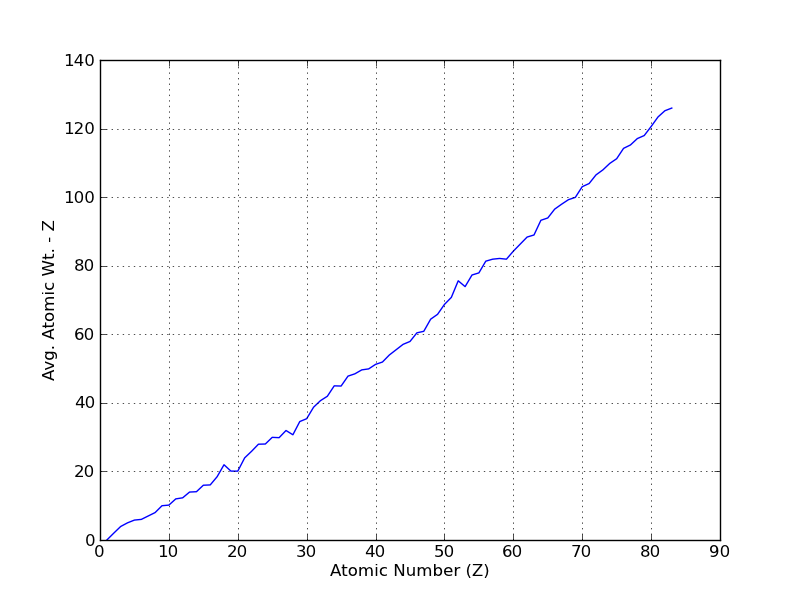
\includegraphics[width=\textwidth]{StabilityBand.png}
	\caption{Average Atomic Weight - Z}
	\label{fig:StabilityBand}
\end{figure}

%%%%%%%%%%%%%%%%%%%%%%%%%%%%%%%%%%%%%%%%%%%%%%%%%%%%%%%
\question{Advanced Topic}{Predicting Radiological Half-Lives}

The prediction of the radiological half-life from first principles was investigated for alpha decay, following the presentation of Dommelen in Quantum Mechanics for Engineers. 
In general there are 10 orders of magnitudes for the half-lives of different nuclei, from nano seconds to quintillions of years (excluding beryllium, which is in the atto second range).
A simple model for alpha decay involves treating the alpha particle as a wavelet packet inside the nucleus.
This packet is trapped inside the nucleus because of the strong nuclear force, but there is always some probability that the particle can tunnel out, this probability is approximated by a transmission coefficient ~\ref{eqn:TransCoeff}.
\begin{align}
	T &\approx e^{-2\gamma_{12}}
	\label{eqn:TransCoeff}
\end{align}
where $\gamma_{12}$ is shown for the case of a high and wide barrier (Coulomb repulsion outside nucleus for wide, strong nuclear force for high).
\begin{align}
	\gamma_{12} &= \frac{1}{\hbar} \int_{x_1}^{x_2} \left | p_c \right | dx \\
	\left | p_c \right | &= \sqrt{2m(V-E)}
\end{align}.
Under this approximation the probability for passing through the barrier is the integration from inside the nucleus to outside the nucleus.
While the probability of a successful tunnel per attempt is quite low the wavelet  bounces around the potential barrier inside the nucleus on the order of $2r_0/v_\alpha$ times per second.
When the integration is preformed there is very good agreement for the even-even nuclei, with slightly less for all nuclei, as shown in Figure ~\ref{fig:AlphaDecayAgreement}.
\begin{figure}[ht]
	\centering
	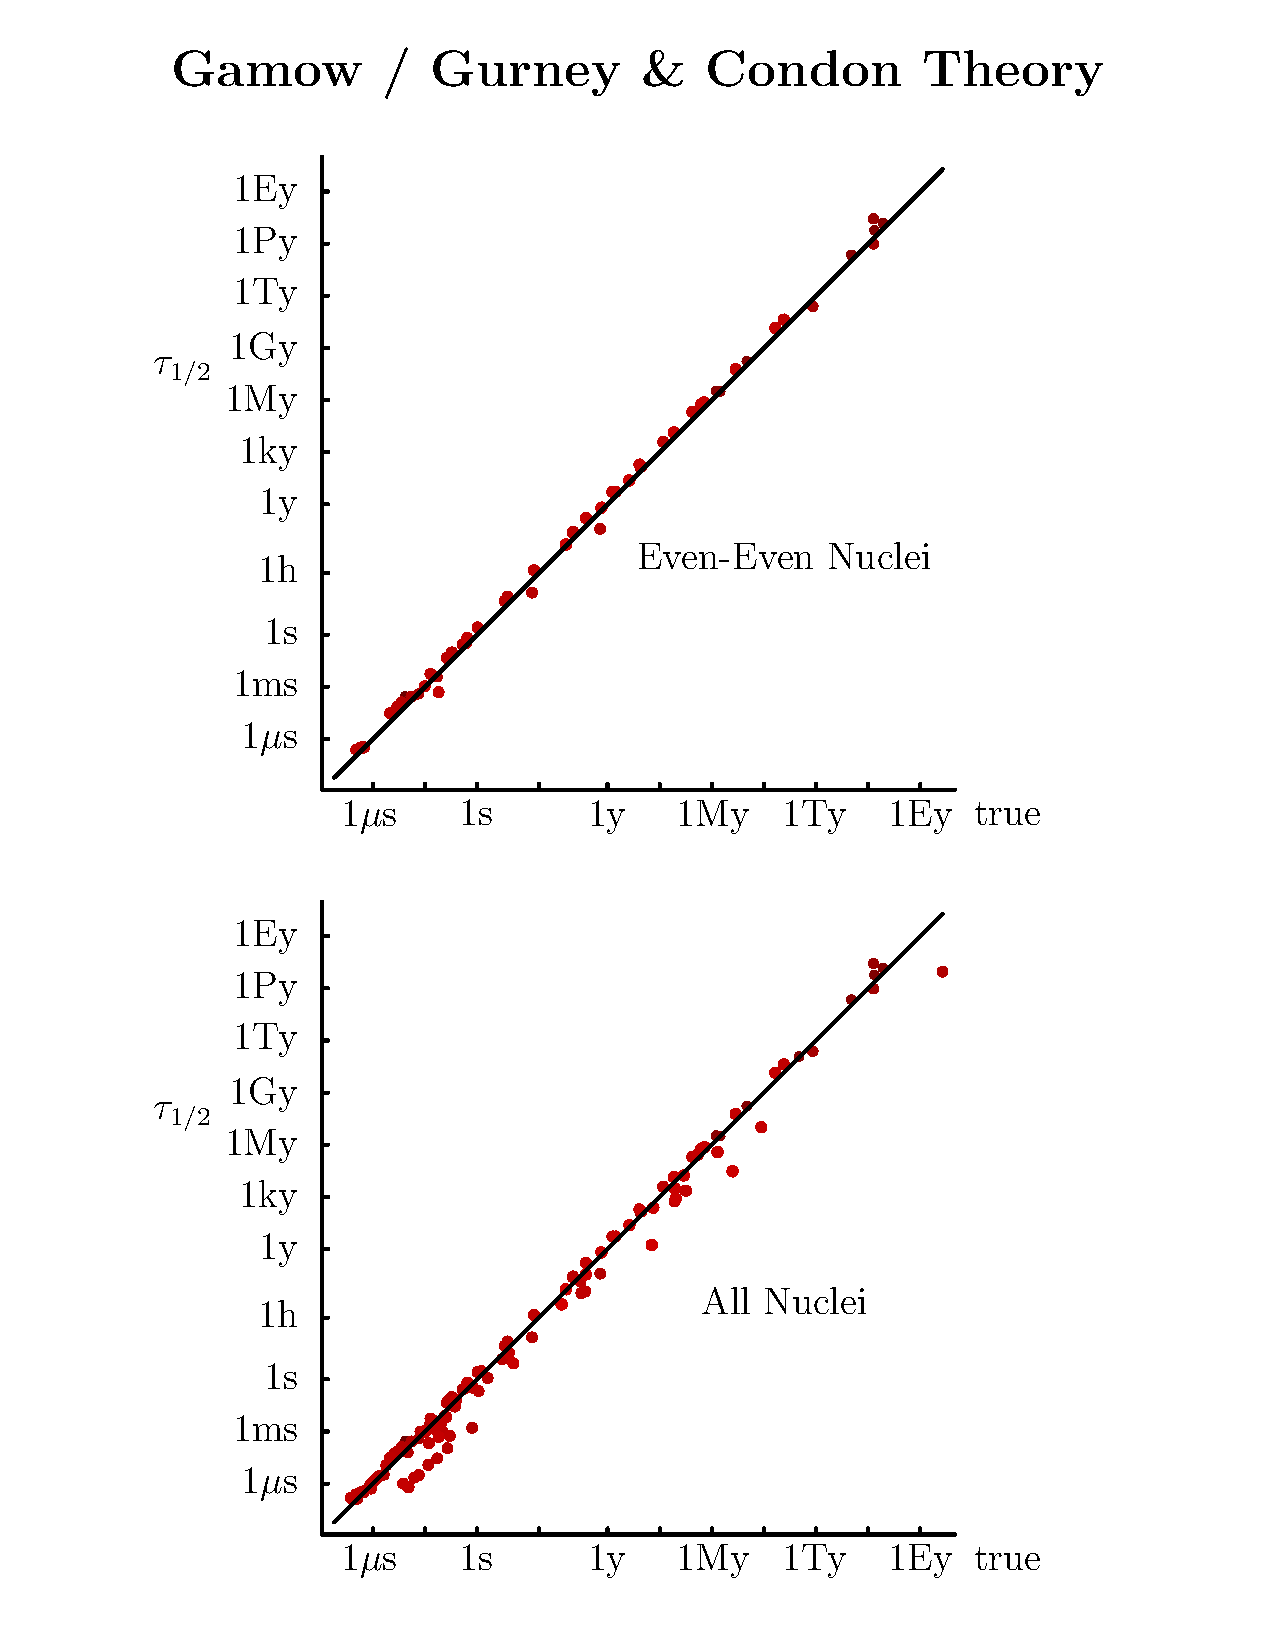
\includegraphics[width=\textwidth]{Gamow_GurneyCondonTheory.pdf}
	\caption{Theory predict half-life agreement.  Reproduced from Dommelen, Quantum Mechanics for Engineers}
	\label{fig:AlphaDecayAgreement}
\end{figure}
\end{document}

